\documentclass[tikz]{standalone}
\usepackage{pgfplots}
\pgfplotsset{compat=1.15}
\usepackage{mathrsfs}
\usetikzlibrary{arrows,calc}
\usepackage{tkz-euclide}
\pagestyle{empty}

\definecolor{AngleClr}{rgb}{0,0.39215686274509803,0}
\definecolor{ShapeClr}{rgb}{0.6,0.2,0}

\begin{document}

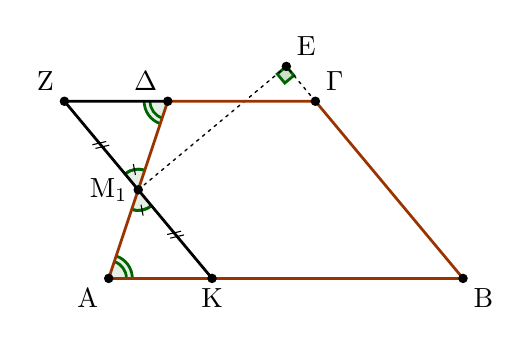
\begin{tikzpicture}[scale=.75]
\tkzSetUpLine[line width=1pt,color=black]
\tkzSetUpPoint[fill=black]

\tkzDefPoints{0/0/A,6/0/B,1/3/D,3.5/3/C}

\tkzDefMidPoint(A,D) \tkzGetPoint{M1}
\tkzDefLine[parallel=through M1](B,C) \tkzGetPoint{x}

\tkzInterLL(M1,x)(A,B)\tkzGetPoint{K}
\tkzInterLL(M1,x)(C,D)\tkzGetPoint{Z}

\tkzDefPointBy[projection=onto B--C](M1) \tkzGetPoint{E}

\tkzFillPolygon[fill=white](A,B,C,D)

\tkzFillAngles[fill=AngleClr,size=.35,fill opacity=0.1](D,M1,Z A,M1,K)
\tkzMarkAngles[line width=1pt,color=AngleClr,size=.35](D,M1,Z A,M1,K)
\tkzMarkAngles[mark=|,mksize=2,line width=1pt,size=.35,color=AngleClr](D,M1,Z A,M1,K)

\tkzFillAngles[fill=AngleClr,size=.4,fill opacity=0.1](Z,D,M1 K,A,M1)
\tkzMarkAngles[line width=1pt,color=AngleClr,size=.3](Z,D,M1 K,A,M1)
\tkzMarkAngles[line width=1pt,color=AngleClr,size=.4](Z,D,M1 K,A,M1)

\tkzMarkRightAngle[line width=1pt, size=.2,color=AngleClr,fill=AngleClr,fill opacity=0.2](M1,E,C)

\tkzDrawSegments(Z,K Z,D)
\tkzDrawSegments[dashed, line width=0.5,dash pattern=on 1pt off 1.75pt](M1,E C,E)

\tkzDrawPolygon[color=ShapeClr](A,B,C,D)
\tkzDrawPoints[size=3](A,B,C,D,K,Z,M1,E)
\tkzLabelPoint[below left](A){$\rm A$}
\tkzLabelPoint[below right](B){$\rm B$}
\tkzLabelPoint[above right](C){$\rm \Gamma$}
\tkzLabelPoint[above left](D){$\rm \Delta$}

\tkzLabelPoint[below](K){$\rm K$}
\tkzLabelPoint[left](M1){$\rm M_1$}
\tkzLabelPoint[above left](Z){$\rm Z$}
\tkzLabelPoint[above right](E){$\rm E$}

\tkzMarkSegments[mark=s||,size=2.3](M1,Z M1,K)

\end{tikzpicture}
\end{document}
